\documentclass[UTF8]{article}
%\usepackage{ctex}
\usepackage{geometry}
\usepackage{cite}
\usepackage{tikz}
\usepackage{xcolor}
\usepackage{listings}
\usepackage{graphicx}
\usetikzlibrary{graphs, positioning, quotes, shapes.geometric}
\usepackage{url}
\usepackage{threeparttable}
%\usepackage{CJK}
\usepackage[colorlinks,
linkcolor=blue,
anchorcolor=blue, 
citecolor=blue,        
]{hyperref}
\usepackage{subfigure}
\usepackage{listings}
\usepackage{ctex}

% 用来设置附录中代码的样式

\lstset{
    basicstyle          =   \sffamily,          % 基本代码风格
    keywordstyle        =   \bfseries,          % 关键字风格
    commentstyle        =   \rmfamily\itshape,  % 注释的风格,斜体
    stringstyle         =   \ttfamily,  % 字符串风格
    flexiblecolumns,                % 别问为什么,加上这个
    numbers             =   left,   % 行号的位置在左边
    showspaces          =   false,  % 是否显示空格,显示了有点乱,所以不现实了
    numberstyle         =   \zihao{-5}\ttfamily,    % 行号的样式,小五号,tt等宽字体
    showstringspaces    =   false,
    captionpos          =   t,      % 这段代码的名字所呈现的位置,t指的是top上面
    frame               =   lrtb,   % 显示边框
}

\lstdefinestyle{python}{
    language        =   python, % 语言选Python
    basicstyle      =   \zihao{-5}\ttfamily,
    numberstyle     =   \zihao{-5}\ttfamily,
    keywordstyle    =   \color{blue},
    keywordstyle    =   [2] \color{teal},
    stringstyle     =   \color{magenta},
    commentstyle    =   \color{red}\ttfamily,
    breaklines      =   true,   % 自动换行,建议不要写太长的行
    columns         =   fixed,  % 如果不加这一句,字间距就不固定,很丑,必须加
    basewidth       =   0.5em,
}
\usepackage[graphicx]{realboxes}
\usepackage{hyperref}

%\ctexset{bibname=}
\geometry{top=1cm}
\begin{document}
	\title{\heiti \textbf {基于孤立森林算法的智能水务分析模型}\vspace{-2em}}
	\date{}
	\author{}
	\maketitle
	\section*{\centering 摘要}
		\par 如何通过有限的水流量数据来判断一个区域的供水系统是否发生故障是一个重要的问题,但是为了解决这个问题需要面对着许多挑战,比如模型的通用性、模型的性能、模型受噪声的影响等,
		可以说这些异常数据的检测至关重要,如何从大量水流量数据中快速找到异常数据是解决这些问题的关键所在,本文将探索并建立合适的模型来进行异常数据的检测,讨论提升模型性能的可能性。
		\par \textbf{对于第一个任务:}首先利用四分位距的方法,判断水流量数据的分布,水流量数据的分布不符合正态分布,因此不采用Z-score来判断异常数据。接着画出箱线图来具象化数据,通过图形可以找到数据的模式、水流量数据的特征,箱线图可以反映上下四分位距,根据四分位距可以确定正常数据的范围,确定判定异常数据的标准,初步找出超出范围之外的异常值,并进一步把他们分为温和异常值和极端异常值。
		\par 但是箱线图只是能帮助初步分析数据,不能作为通用模型,箱线图依旧存在着无法准确检测异常数据的问题,因为箱线图有时会将很多正常的数据判断为异常数据。
		\par \textbf{对于第二个任务:}为了建立合适的通用模型,文章接下来基于数据的特点进一步选取合适的算法,经过对数据模式的分析,抓住数据的特点,考虑了孤立森林算法,文章讨论了孤立森林算法是否适用于水流量数据的异常检测,并最终决定采用孤立森林算法来检测异常数据,后续的讨论中可以看到,孤立森林算法检测的异常值是符合上述异常值检测标准的。
		孤立森林算法是一种无监督学习算法,可以很好地快速处理大量数据,鲁棒性好,还能够将噪声的影响降到最低,在没有异常数据也能够进行训练。基于数据的特点,选择合适的数据集——异常数据较少、异常值差别较大进行训练。然后在所有的八个虚拟地区进行检测,得到结果并分析数据特点与数据模式。
		\par \textbf{对于第三个任务:}本文希望衡量该模型的优劣,训练所得模型的好坏取决于训练集的划分和参数的选取。可以通过箱线图对数据进行的分析来划分训练集,然后在测试集上进行测试,通过测试结果来计算精确度和F1-Score等指标,用于评判该模型优劣,然后指出应该如何优化该模型,存在哪些可能性可以提升模型的性能。
		\\ 
		\\
		\textbf{\centering 关键词: IQR、非正态分布、箱线图、孤立森林算法}
		\newpage
	\section{问题重述}
		\subsection{问题背景}
		\par 供水系统在我们的日程生活中至关重要,但是供水系统有时会发生各种各样的故障,从而导致漏水的发生,这是一个大问题。在这样的背景下,电磁流量计应运而生,用于测量流量以及监测漏水,一种方法是获取某一区域输入和输出水流量的插值加以评价。 
		\par 如今已经有许多基于流量数据的分析方法,但是还有一些挑战存在,比较重要的三个:首先是需要设计一个通用模型来了解流量计的数据模式,然后是如何更加快速地检测流量异常,最后一个挑战是如何应对噪声的影响。\cite[C1]{znswxxh}
		\subsection{具体问题}
		\par 您的团队需要设计一个模型来应对上述挑战,需要对给定数据进行清理,开发异常检测模型,并优化模型,数据是八个不同虚拟区域的输入水流量和输出水流量之差。具体的任务有:

		\begin{itemize}
			\item 分析数据模式,建立检测异常的标准
			\item 建立通用模型对八个区域进行异常值检测
			\item 测试模型并解释建模和异常值检测的结果
		\end{itemize}
		解决这些问题的关键是找到一个合适的异常数据检测算法。
	\section{数据模式分析与异常检测标准的确立}	
		\subsection{数据概览分析}
			\par 题目所给的数据来自于八个不同的虚拟地区,每个地区的流量差值是一个与时间相关的变量,这些值中既有正数,也有负数。大部分流量之差的绝对值都在10以内,如果发现绝对值过大,则可初步认为该数据是异常数据。流量数据随着时间的变化而变化,不同地区流量数据随时间变化的规律也各不相同。
			\par 首先判断各个地区的数据是否满足正态分布,采用四分位距的方法判断是否满足或者接近于正态分布,如果符合正态分布,则可以使用Z-score判断数据是否异常,如果不符合,则需要考虑其他的方法。
			\par 计算可得八个虚拟地区输入和输出水流量之差的四分位距:
			\begin{table}[!ht]
				\centering
				\resizebox{0.8\textwidth}{!}
				{
					\begin{tabular}{|l|l|l|l|l|l|l|l|l|}
					\hline
						region\_1 & region\_2 & region\_3 & region\_4 & region\_5 & region\_6 & region\_7 & region\_8 \\ \hline
						3.802019768 & 1.108408668 & 1.2881612 & 0.678413944 & 4.157332959 & 4.746437346 & 6.514955518 & 1.616935081 \\ \hline
					\end{tabular}
				}
			\end{table}
			\\可见并不满足正态分布的要求,因此不能采用Z-score判断数据是否异常。对于不满足正态分布的数据,可以使用箱线图进行异常数据的检测。
			\newpage
			\subsection{利用箱线图进行数据分析并检测异常数据}
			下面是根据八个地区数据所作出的箱线图\ref{Box},可以初步比较直观地对数据进行分析,也可以看出哪些是异常数据:
			\begin{figure}[!ht]
				\centering %表示居中
				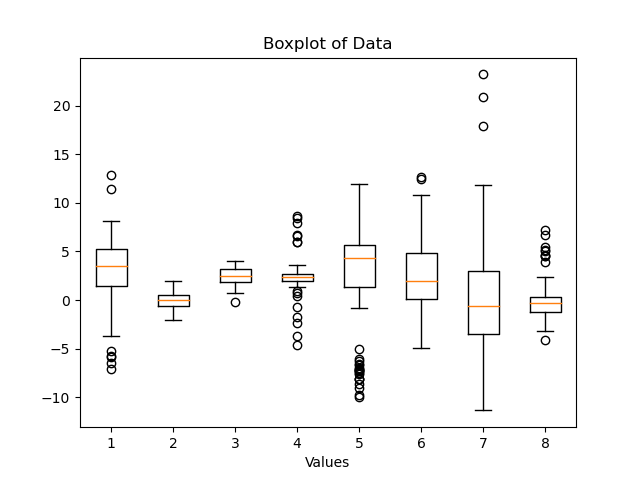
\includegraphics[height=4.5cm,width=9.5cm]{pictures/BoxPlot.png}
				% [height=4.5cm]表示高度
				%[width=9.5cm]表示宽度
				%{111.eps}表示eps格式的图片,名为111
				\caption{八个虚拟地区的箱线图}
				%图片的名称
				\label{Box}
				%图片的标签,用于文章中的引用,注意到标签的数字与实际文章显示的数字可能不同
			\end{figure}
			\par 从箱线图中,我们可以直观地看出每个地区的中位数、四分位数、异常数据以及数据的集中程度,箱线图较短的区域如2、3、4、8号地区数据集中程度就比较好。
			也可以用箱线图判断不同地区的数据趋向于哪种分布,比如区域三更趋向于正态分布,而其他区域的分布都有更多的偏移,既有左偏的分布又有右偏的分布,这些都可以直观地从箱线图中看出来。
		\subsection{异常检测标准的确立}
			已经使用了箱线图的办法,因此类似于正态分布中的3$\sigma$原则,可以借助第一、第三四分位数和四分位距IQR来对异常数据进行判断,对于每一个区域,
			找出他的第一和第三四分位数,然后先计算IQR:
			$$
			IQR=Q_3-Q_1
			$$
			然后计算内限范围:
			$$
			R_1=\left[ Q_1-1.5IQR,Q_3+1.5IQR \right] 
			$$
			以及外限范围:
			$$
			R_2=\left[ Q_1-3IQR,Q_3+3IQR \right] 
			$$
			处于内限范围以外的均为异常值,其中在外限以内的是温和异常值,在外限以外的是极端异常值。第4、5、8区域的异常值较多,第4区域的异常值最多,可以推测该地区的水流计发生了故障。
	\section{建立通用异常检测模型}
			\subsection{通用模型算法的选取与建立}
			\par 通过箱线图进行分析以后,可以初步分析数据特征、找出异常数据,但是为了建立通用模型来检测异常数据,箱线图显然并不合适,箱线图只适合于反映数据的一些基本特征,在检测异常数据上不合适,比如区域4数据显然大部分都是正常的,然而箱线图却看出很多异常数据,这体现了箱线图的一些问题,那就是会检测出过多的异常数据。
			\par 通过上述的箱线图可知,每个区域异常值的占比都很低,且异常数据和正常数据的差别较大。因此可以采用孤立森林算法建立通用模型来进行异常值的检测。
			\par 孤立森林算法不需要对数据的分布做出假设,也不需要预处理数据,即使没有异常数据也能进行训练,这种算法大大降低了噪声的影响,训练所得模型可以快速处理大量数据并准确检测异常值\cite[iForest]{liu2008isolation}
			\par 下面展示了二维高斯分布中应用该方法找出孤立数据\cite{wikiif}
			\begin{figure} [!h]
				\centering
				\subfigure[\label{normal}]{
					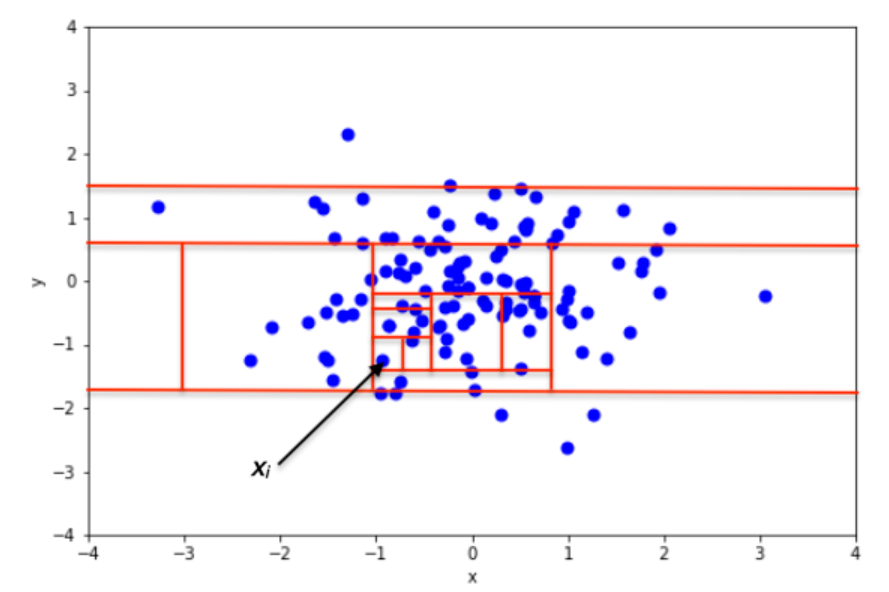
\includegraphics[scale=0.4]{pictures/iforest_example.png}}
				\subfigure[\label{abnormal}]{
					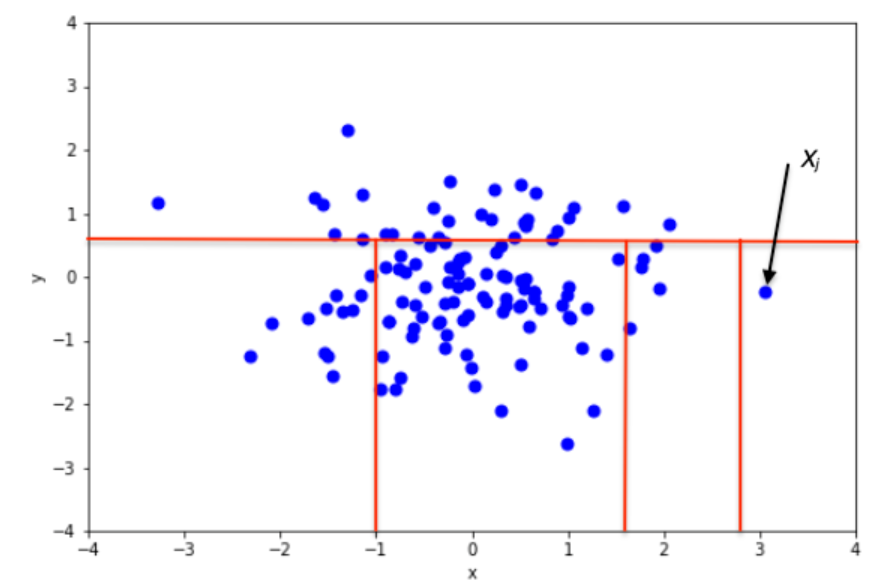
\includegraphics[scale=0.4]{pictures/wikiifi.png}}
				\caption{应用孤立森林算法的例子}
				\label{example}
			\end{figure}
			\\图\ref{sub@normal}反映了正常数据的划分情形,而图\ref{sub@abnormal}反映了孤立点也就是异常数据的情形。
			\par 算法是通过构建多棵iTree(isolation Tree)来实现的,通过随机选择数据中的某些特征,并在这些特征的范围内随机选择一个划分点,将数据分配到树的不同分支上,直到每个叶子节点中只包含一个或少量的数据点。由于异常点很少,所以它们往往需要更少的分割才能被隔离到树的较深层。因此,异常点在孤立森林中的路径长度通常比正常点短。
			由于每个数据点都可以用路径长度来表示,因此可以将路径长度作为异常度量,即路径长度越小,则数据点越可能是异常值。
			\par 路径长度的计算公式如下:
			$$
			\mathrm{h}\left( \mathrm{x} \right) =\mathrm{e}+\mathrm{c}\left( \mathrm{T}.\mathrm{size} \right) 
			$$
			然后就可以计算异常分了,有时候计算异常分有不同方式,因此划分的方式也有所不同,但不会影响结果,比如scikit-learn中异常值由负数表示,正数意味着正常,下面是一种常规的归一化计算方法:
			$$
			\mathrm{s}\left( \mathrm{x},\mathrm{n} \right) =2^{-\frac{\mathrm{E}\left( \mathrm{h}\left( \mathrm{x} \right) \right)}{\mathrm{c}\left( \mathrm{n} \right)}}
			$$
			得分接近于1时,路径长度非常小,数据就会被孤立,因此较高的异常值路径长度较低。
			\subsection{训练集的划分与训练参数的设置}
			\par 基于孤立森林法的特点,为了提高训练效果,提高模型的准确性、稳定性,应当选取异常数据较少地区的数据进行训练,另外,也要选取合适的参数。\cite{zhihuiif1}
			\par 选取异常数据较少且异常数据差异较大的地区的数据作为训练集,选取区域7来进行训练,完成训练后可以在八个地区上进行测试。
			\newpage \par 在设定参数之前,先列举一下重要参数:
			\begin{itemize}
				\item n\_estimators: iTree的个数
				\item max\_samples: 构建子树的样本数
				\item contamination: 异常数据所占的比例
				\item max\_features: 每个子树的特征数
				\item bootstrap: 采样是有放回还是无放回
				\item n\_jobs: 作业数量
				\item random\_state: 训练的随机性 
				\item verbose: 训练中打印日志的详细程度
				\item warm\_start: 是否重用上次调用的结果去fit
			\end{itemize}
				\par 参数设置考虑如下:
				\\n\_estimators,这个参数越大,算法的运行时间就越长,但是模型的性能也有可能提高。这里设置为100,如果不满足性能要求可以继续提高。
				\\max\_samples,每个随机树使用的样本数量。这个参数可以控制随机树的分支程度。设置为"auto",这样算法会使用全部数据样本。
				\\max\_features,每个随机树使用的最大特征数量。这个参数可以控制随机树的分支程度。设置为"auto",这样算法会使用全部特征。
				\\contamination,异常样本比例,提高该参数将使得标准更为严格,可能会使很多正常数据被判断为异常数据,因此设为0.05即可
				\begin{itemize}
					\item n\_estimators = 100
					\item max\_samples = 'auto'
					\item contamination = 0.05
					\item max\_features = 1
					\item bootstrap = False
					\item n\_jobs = None
					\item random\_state = None 
					\item verbose = 0
					\item warm\_start = False
				\end{itemize}
				大部分均为默认参数设置,在这样的参数设定下,调用sklearn的IsolationForest模块进行训练。
	\section{模型的测试与评价}
			\subsection{利用模型检测各个区域的异常数据}
			在区域7数据上完成数据的训练后,对每个区域进行检测,检测结果如下表所示:
			\begin{table}[!ht]
				\centering
				\resizebox{0.8\textwidth}{!}
				{
				\begin{tabular}{|l|l|l|l|l|l|l|l|}
				\hline
					region1 & region2 & region3 & region4 & region5 & region6 & region7 & region8 \\ \hline
					12.8423647800  & none & none & 11.2105270500  & 11.4587055000  & 12.61496345 & 23.2090330700  & none \\ \hline
					11.3752904700  & ~ & ~ & ~ & 11.9137123000  & 12.4629461600  & 11.8275897600  & ~ \\ \hline
					~ & ~ & ~ & ~ & ~ & ~ & -11.3403016100  & ~ \\ \hline
					~ & ~ & ~ & ~ & ~ & ~ & 20.8840092400  & ~ \\ \hline
					~ & ~ & ~ & ~ & ~ & ~ & 17.9267807800 & ~ \\ \hline
				\end{tabular}
				}
			\end{table}
			\\这个结果与箱线图的结果有较大不同,这是因为箱线图对数据的要求过于严格,以至于很多正常的数据都在箱线图上被判断成了异常数据。
			\\下面给出了是每个区域检测结果的散点图,可以更加直观地看出数据的分布以及异常数据是如何被检测出来的。
			\newpage
			\begin{figure}[!ht]
				\centering
				\subfigure[\label{scatter1}]{
					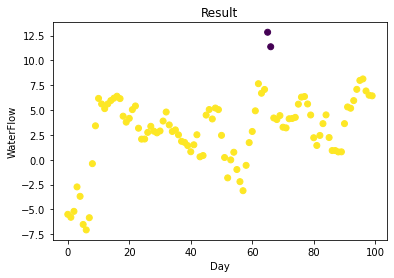
\includegraphics[scale=0.4]{pictures/ScatterRegion_1.png}}
				\subfigure[\label{scatter2}]{
					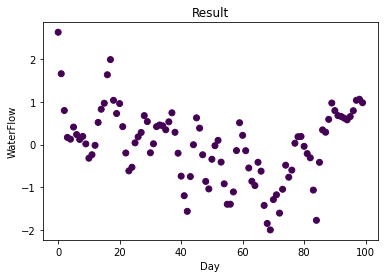
\includegraphics[scale=0.4]{pictures/ScatterRegion_2.png}}
				\subfigure[\label{scatter3}]{
					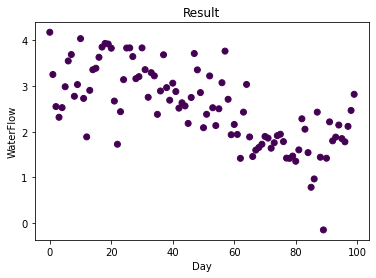
\includegraphics[scale=0.4]{pictures/ScatterRegion_3.png}}
				\subfigure[\label{scatter4}]{
					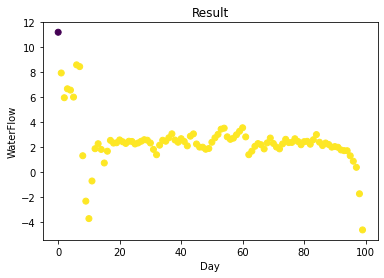
\includegraphics[scale=0.4]{pictures/ScatterRegion_4.png}}
				\subfigure[\label{scatter5}]{
					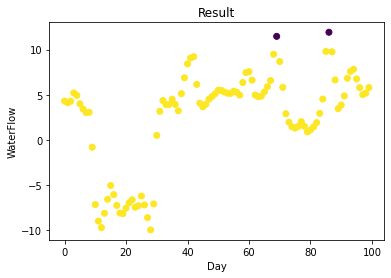
\includegraphics[scale=0.4]{pictures/ScatterRegion_5.png}}
				\subfigure[\label{scatter6}]{
					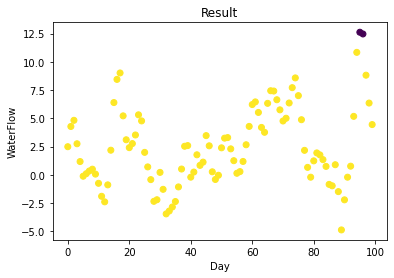
\includegraphics[scale=0.4]{pictures/ScatterRegion_6.png}}
				\subfigure[\label{scatter7}]{
					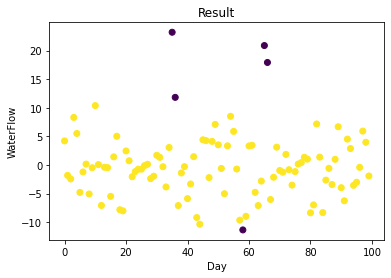
\includegraphics[scale=0.4]{pictures/ScatterRegion_7.png}}
				\subfigure[\label{scatter8}]{
					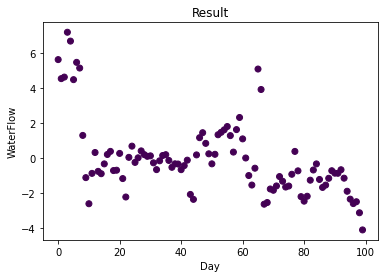
\includegraphics[scale=0.4]{pictures/ScatterRegion_8.png}}
				\label{scatter}
				\caption{孤立森林检测散点图}
			\end{figure}
			说明本文建立的模型所检测的异常数据还是少数,异常数据在所有数据中占比较低,这也是符合日常生活的,相比之下,前文的箱线法的结果就比较违背常理了——异常数据过多。
			\subsection{再次测试模型并评价各项指标}
				\par 现在需要一些指标来对模型进行评价,根据应用场景要求,模型完成的实际上是一个分类的任务,可以用精确度来衡量,但这不够全面,因为另一个指标——召回率,在
				这个模型的评价中也很重要,所以应当考虑综合了精确度和召回率的指标——F1-Score来对模型进行评价。
				\par 于是再次测试,得到每个区域检测的精确度和F1-score指标
				\begin{table}[!ht]
					\centering
					\resizebox{0.9\textwidth}{!}{
					\begin{tabular}{|l|l|l|l|l|l|l|l|l|}
					\hline
						  &region1 & region2 & region3 & region4 & region5 & region6 & region7 & region8 \\ \hline
						Accuracy & 0.980000  & 1.000000  & 1.000000  & 0.990000  & 0.980000  & 0.970000  & 0.950000  & 1.000000  \\ \hline
						F1-Score & 0.989899  & 1.000000  & 1.000000  & 0.994974  & 0.989899  & 0.984772  & 0.974359  & 1.000000 \\ \hline
					\end{tabular}
					}
				\end{table}
			可见,该模型对于水流量异常数据的检测效果很好,无论是精确度还是F1-Score都比较理想。
				\subsection{模型优化的方面}
				\par 虽然测试结果比较好,但是该模型可能仍然有一定的局限性,首先因为只有100天的数据,其次并且训练数据集的数据模式也并不一定是最合适的,
				如果有更好的数据集,也就是异常数据更少、异常值偏差更大的数据集,那么训练出来的模型检测将会更加准确。
				\par 另一方面,可以通过调整训练的参数来提升模型的性能,参数对于模型训练效果的影响是复杂的,只有不断试验,结合原理,不断改变参数的值,才能找到更合适的参数。有时可能会耗时更多,计算量更大,但有望提高模型的性能。
				\par 此外,这仅仅只有水流量这一个因素,故障的检测还可以考虑更复杂的物理因素,比如水压、流速等等,虽然可能会使模型更加复杂,但却能从本质上提高模型的精确度,带来质的飞跃。
	\newpage
	\bibliographystyle{unsrt}
	\bibliography{refs.bib}
	\newpage
	\section*{附录}
	\subsection*{I 程序源代码}
	绘制箱线图:
		\begin{lstlisting}[language=Python]
	import pandas as pd
	import matplotlib.pyplot as plt

	data = pd.read_csv('workspace\data.csv')

	fig, ax = plt.subplots()
	ax.boxplot(data)

	ax.set_title('Boxplot of Data')
	ax.set_xlabel('Values')

	plt.show()
		\end{lstlisting}
		训练并测试模型,绘制散点图
		\begin{lstlisting}[language=Python]
	import numpy as np
	import pandas as pd
	from sklearn.ensemble import IsolationForest
	import matplotlib.pyplot as plt

	data = pd.read_csv('data.csv')

	Xtrain = data['region_7'].values.reshape(-1, 1)
	Xtest = data['region_1'].values.reshape(-1, 1)

	model = IsolationForest(n_estimators=100, contamination=0.05)

	model.fit(Xtrain)

	y_pred = model.predict(Xtest)


	outliers = Xtest[np.where(y_pred == -1)]

	print('异常值:', outliers)

	plt.scatter(np.arange(len(Xtest)), Xtest, c=y_pred, cmap='viridis')

	plt.xlabel('Day')
	plt.ylabel('WaterFlow')
	plt.title('Result')

	plt.show()
	\end{lstlisting}
	评价模型	
	\begin{lstlisting}[language=Python]
	import numpy as np
	import pandas as pd
	from sklearn.ensemble import IsolationForest
	import matplotlib.pyplot as plt
	from sklearn.metrics import accuracy_score, f1_score

	data = pd.read_csv('data.csv')


	Xtrain = data['region_7'].values.reshape(-1, 1)
	Xtest = data['region_8'].values.reshape(-1, 1)

	model = IsolationForest(n_estimators=100, contamination=0.05)

	model.fit(Xtrain)

	y_pred = model.predict(Xtest)

	outliers = Xtest[np.where(y_pred == -1)]

	print('异常值:', outliers)
	accuracy = accuracy_score(y_true=np.ones(len(Xtest)), y_pred=y_pred)
	print('预测准确率:', accuracy)
	f1score = f1_score(y_true=np.ones(len(Xtest)), y_pred=y_pred)
	print('F1分数:', f1score)	
	\end{lstlisting}
	\subsection*{II 支撑材料文件列表}
	以下是建模过程中用到的文件合集
	\begin{itemize}
		\item 数据文件.xls:原始的数据文件
		\item sourcecode.rar:建模用到的代码文件、运行代码所需的数据文件和记录结果用的文件
		\item pictures.rar:写论文用到的图片,生成的图片
	\end{itemize}
\end{document}